\begin{frame}{Hello from IRIS-HEP and Scikit-HEP!}
  \begin{columns}
    \column{0.6\textwidth}
    \Large
    % \begin{itemize}
    \begin{itemize}\setlength{\itemsep}{0.5 cm}
      \item We're members of the \href{https://iris-hep.org/}{Institute for Research and Innovation in Software for High Energy Physics (IRIS-HEP)} and the \href{https://scikit-hep.org/}{Scikit-HEP} community project developing a Pythonic data analysis ecosystem for HEP
      \item Goals: Empower analysts with modern data science stacks and provide powerful libraries for building expressive workflows
    \end{itemize}
%
    \column{0.4\textwidth}
    \begin{figure}
        \begin{center}
            
\includegraphics[width=0.9\linewidth]{iris-hep-logo-long.pdf}
            
\includegraphics[width=0.8\linewidth]{scikit-hep-logo.pdf}
        \end{center}
    \end{figure}
  \end{columns}
\end{frame}

% shows the rapid adoption of Python for analysis in recent years
\begin{frame}{Rapid rise of Python for analysis in HEP}
\vspace{0.25 cm}
\textcolor{darkblue}{Source: ``\mintinline{python}{import XYZ}'' matches in GitHub repos for users who fork CMSSW.}

\vspace{0.2 cm}
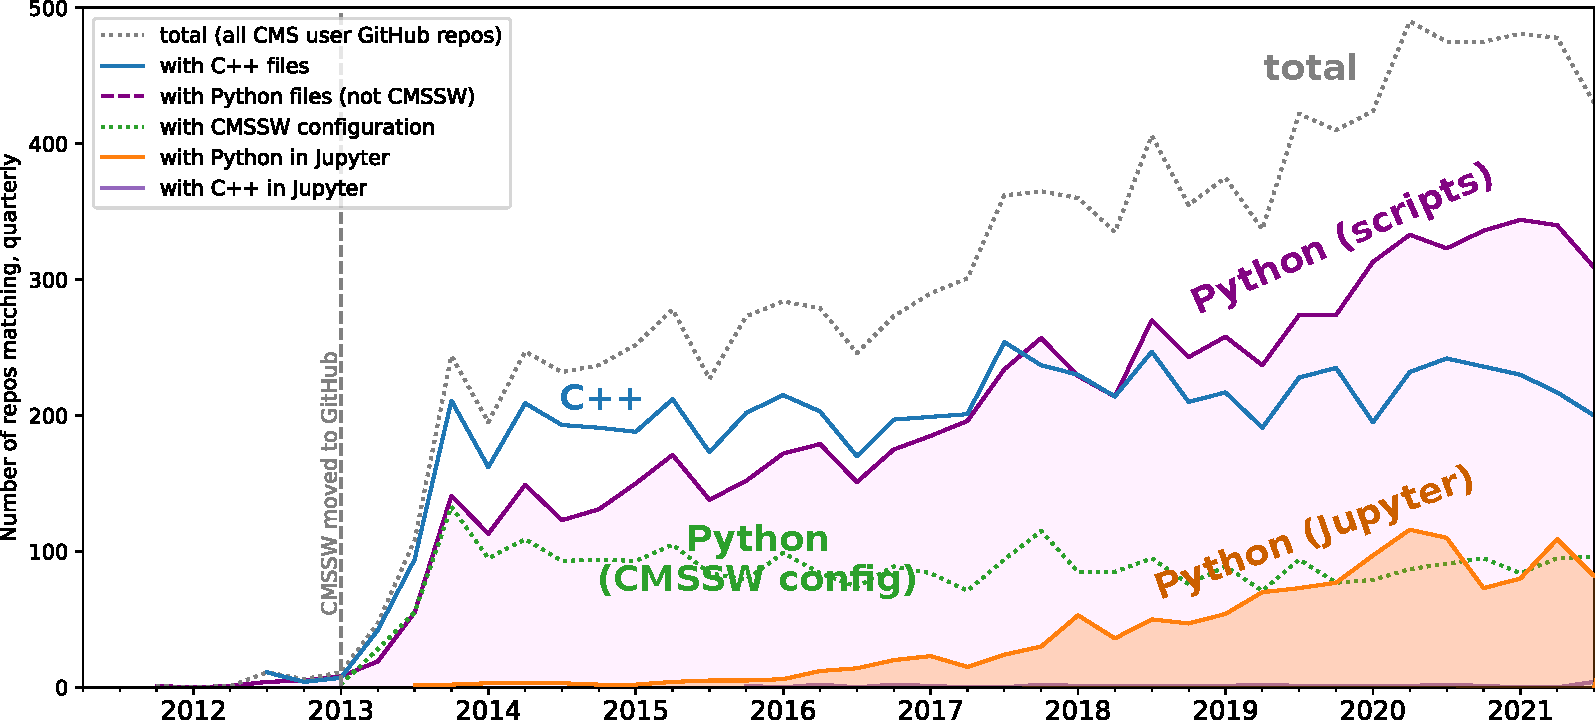
\includegraphics[width=\linewidth]{github-language-fullstudy-for-review.pdf}
\textcolor{darkblue}{\tiny (CMSSW is the CMS experiment's ``offline'' software framework)}
\end{frame}

\begin{frame}{Explosion of Scientific Python (NumPy, etc.) use recent since 2018}
\vspace{0.25 cm}
\textcolor{darkblue}{Source: ``\mintinline{python}{import XYZ}'' matches in GitHub repos for users who fork CMSSW.}

\vspace{0.2 cm}
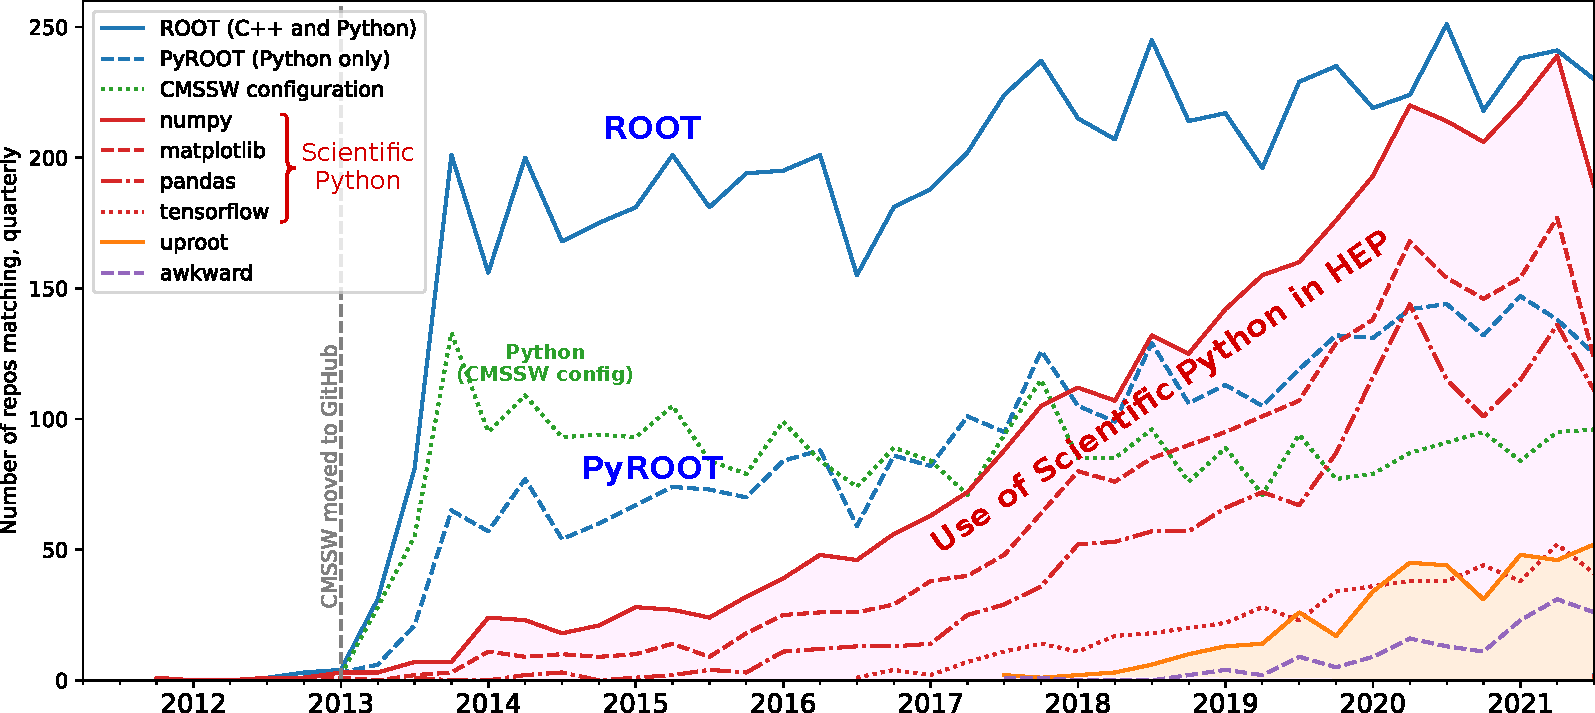
\includegraphics[width=\linewidth]{github-package-fullstudy-for-review.pdf}
\end{frame}

\begin{frame}{Growth tightly coupled to the rise of Scikit-HEP supported by IRIS-HEP}
\vspace{0.25 cm}
\textcolor{darkblue}{Source: ``\mintinline{bash}{pip install XYZ}'' download rate for MacOS/Windows (no batch jobs).}

\vspace{0.1 cm}
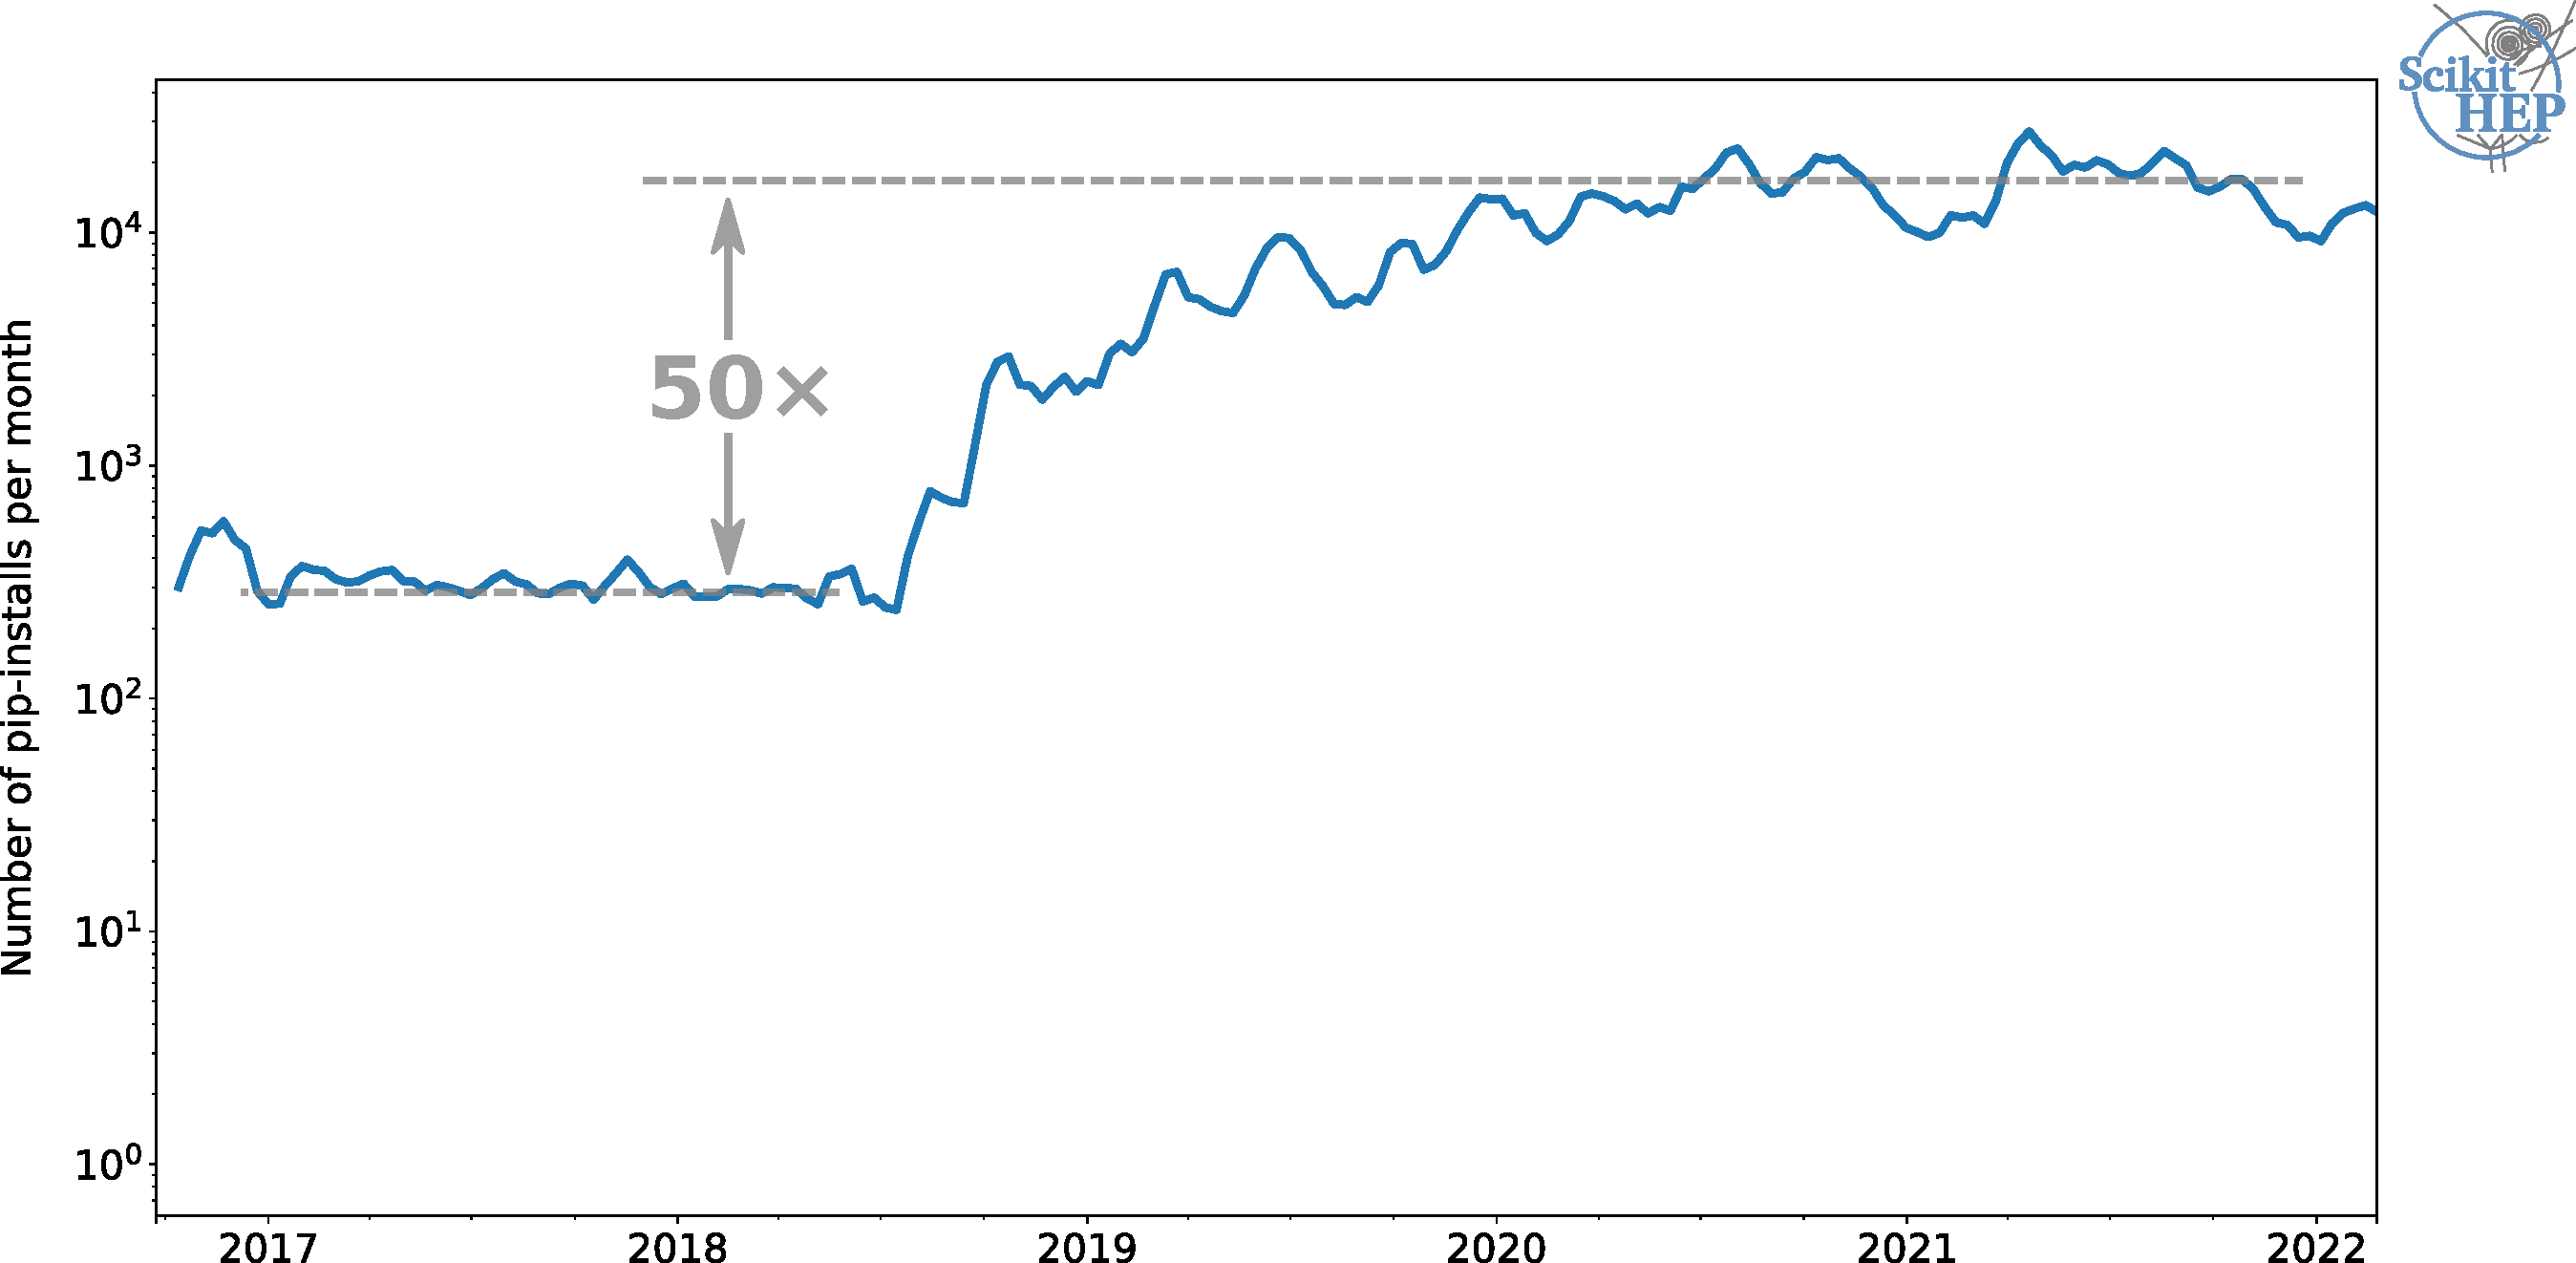
\includegraphics[width=\linewidth]{pip-macwin-scikithep-log-combined.pdf}
\end{frame}

\begin{frame}{Growth tightly coupled to the rise of Scikit-HEP supported by IRIS-HEP}
\vspace{0.25 cm}
\textcolor{darkblue}{Source: ``\mintinline{bash}{pip install XYZ}'' download rate for MacOS/Windows (no batch jobs).}

\vspace{0.1 cm}
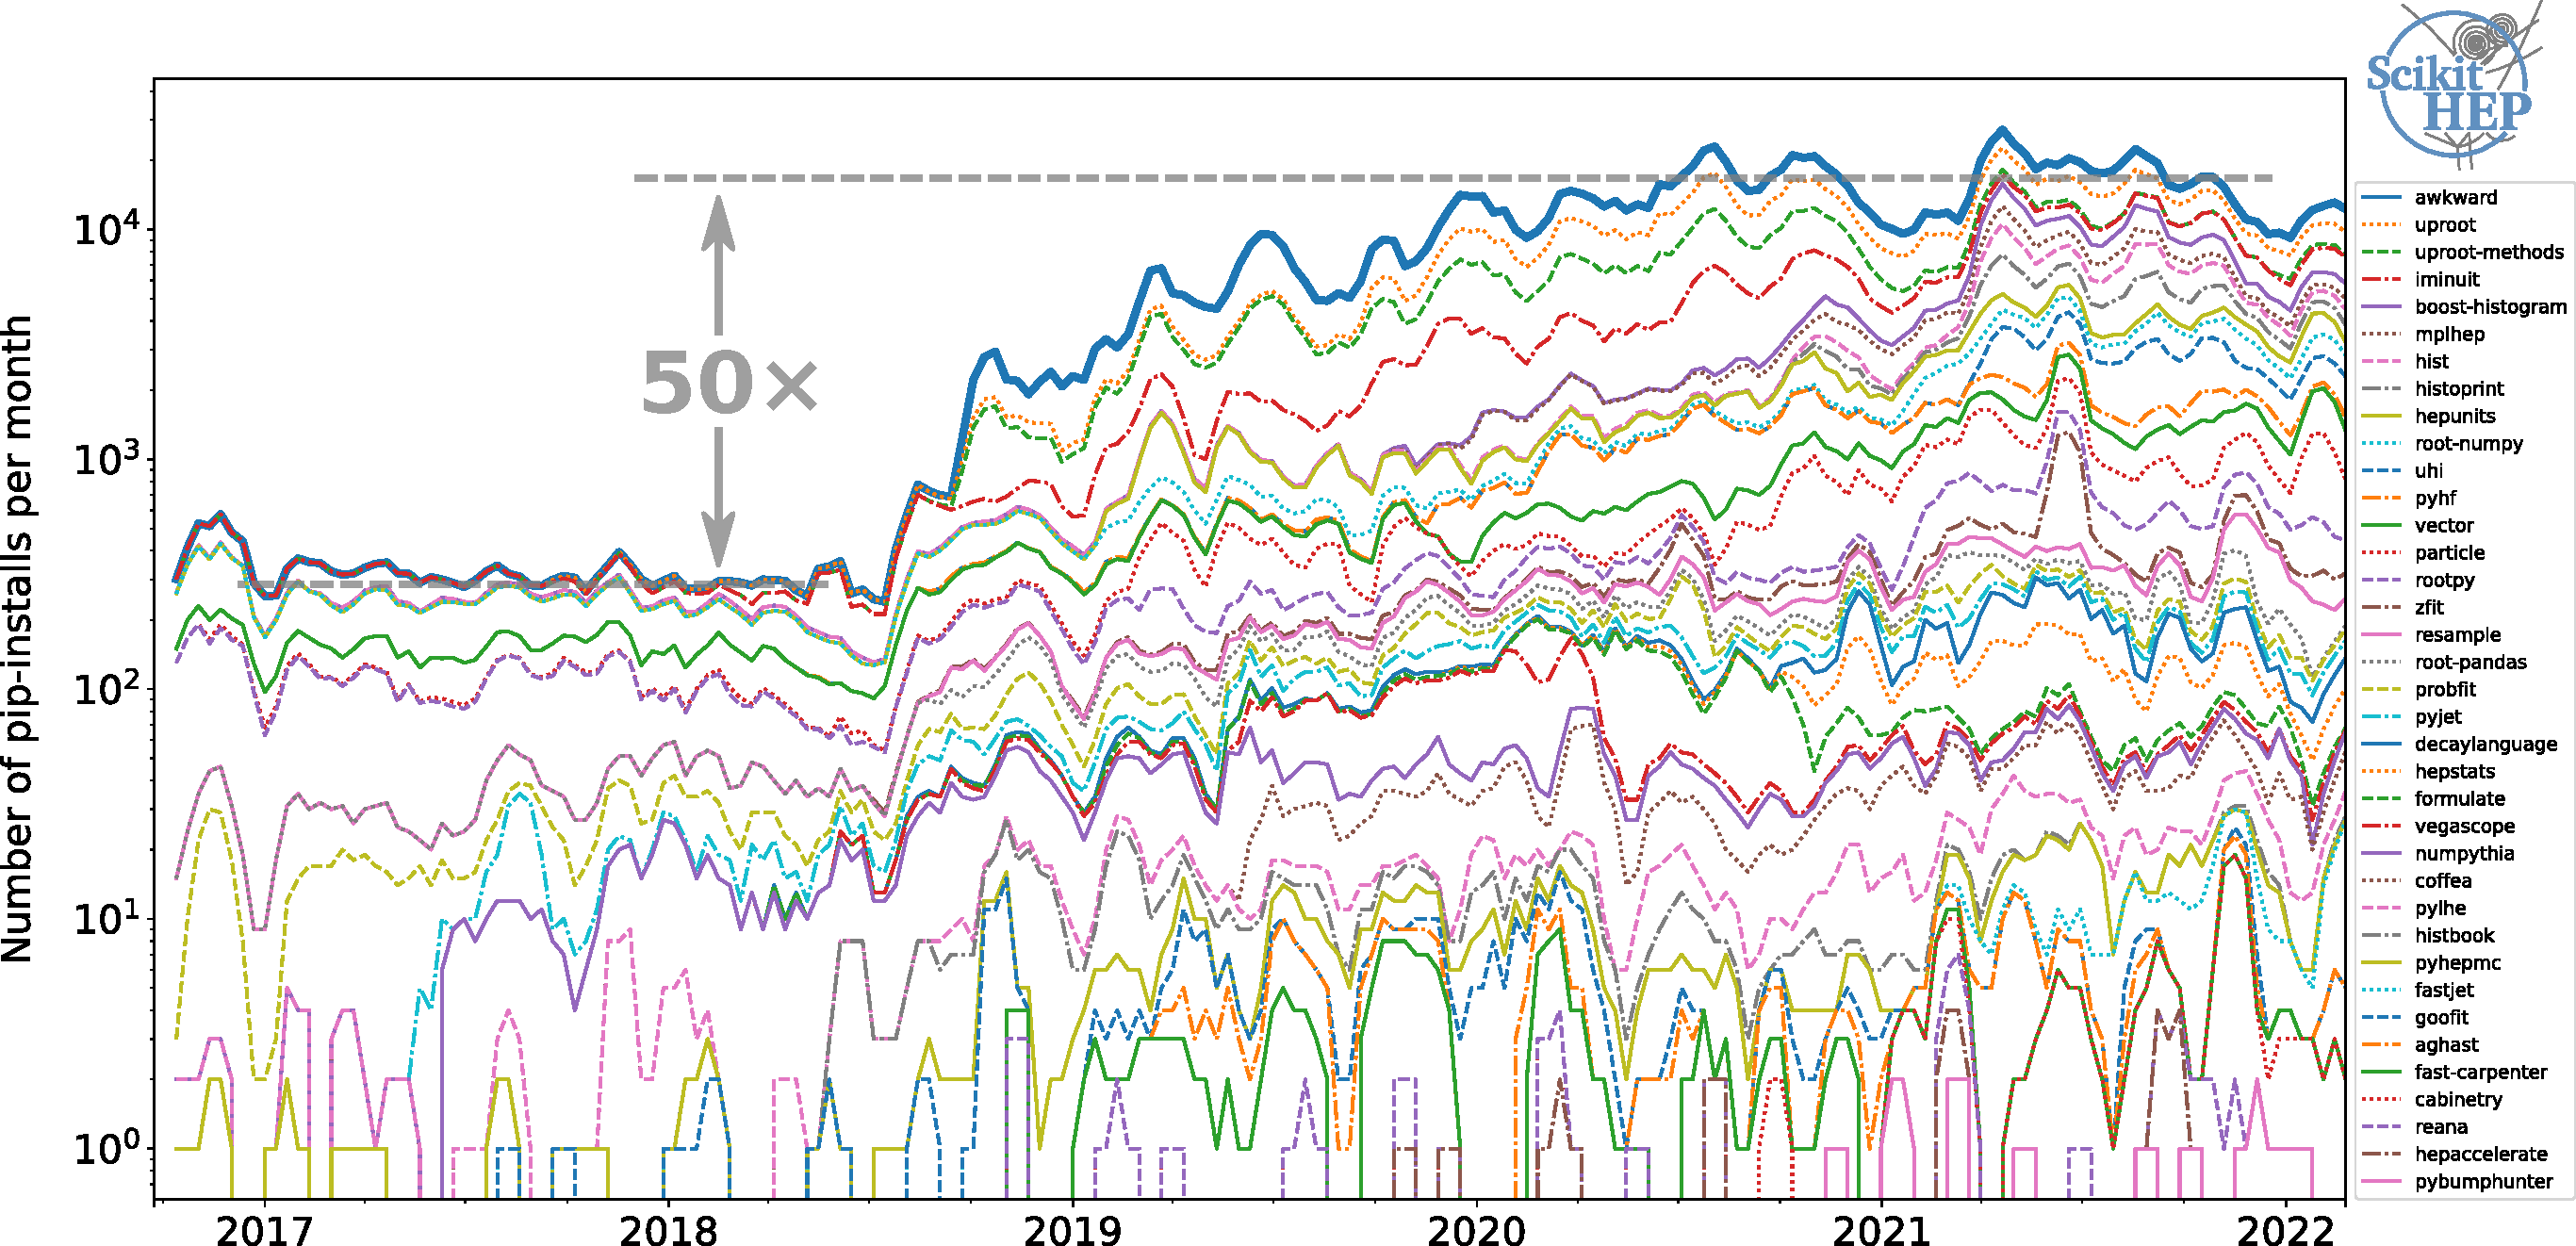
\includegraphics[width=\linewidth]{pip-macwin-scikithep-log-by-package.pdf}
\end{frame}

\begin{frame}{Ecosystems}
\vspace{0.25 cm}
\begin{center}
    {\small In his \href{https://youtu.be/ZyjCqQEUa8o}{PyCon 2017 keynote}, Jake VanderPlas gave us the iconic ``PyData ecosystem'' image}
\end{center}

\vspace{0.1 cm}
\begin{figure}
    \begin{center}
        \href{https://coiled.io/blog/pydata-dask/}{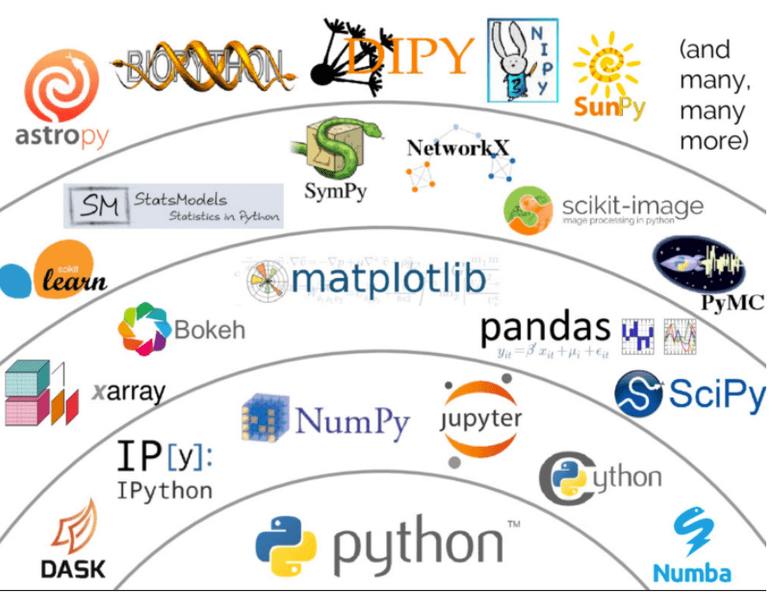
\includegraphics[width=0.60\linewidth]{pydata-ecosystem-pycon-2017.png}}
    \end{center}
\end{figure}
\end{frame}

\begin{frame}{Pythonic ecosystem for particle physics}
\vspace{0.25 cm}
\begin{center}
    {\small Working view of a PyHEP ecosystem (Scikit-HEP and IRIS-HEP supported projects)}
\end{center}

% \vspace{0.1 cm}
\begin{figure}
    \begin{center}
        \href{https://indico.cern.ch/event/1140031/}{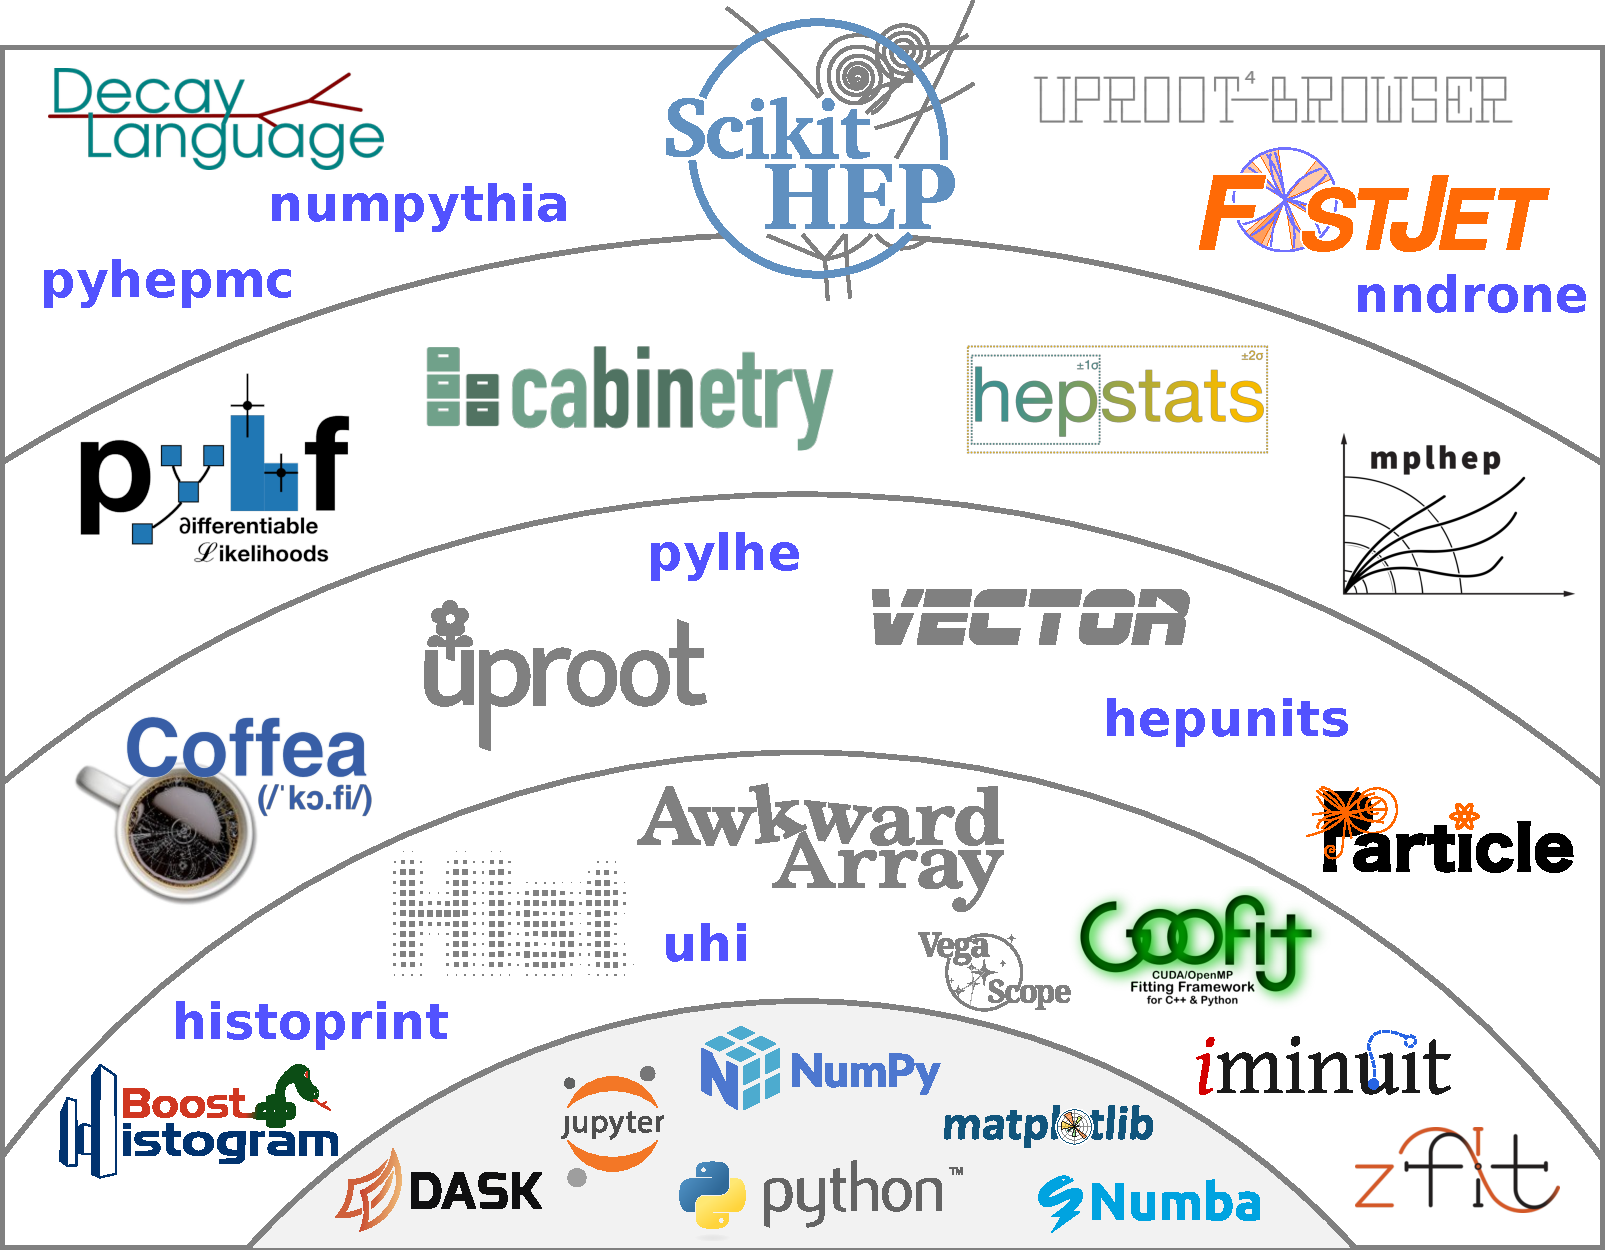
\includegraphics[width=0.60\linewidth]{shells-hep.pdf}}
    \end{center}
\end{figure}
\end{frame}

\begin{frame}{Built with intentionality and interoperability}
  \begin{columns}
    \column{0.45\textwidth}
    \begin{enumerate}\setlength{\itemsep}{0.5 cm}
      \item[5] HEP-specific UI applications or packaged algorithms
      \item[4] HEP-specific for common problems
      \item[3] HEP-specific, foundational
      \item[2] needed to create, but not really HEP-specific
      \item[1] non-HEP software we depend on
    \end{enumerate}
%
    \column{0.55\textwidth}
    \begin{figure}
        \begin{center}
            \href{https://indico.cern.ch/event/1140031/}{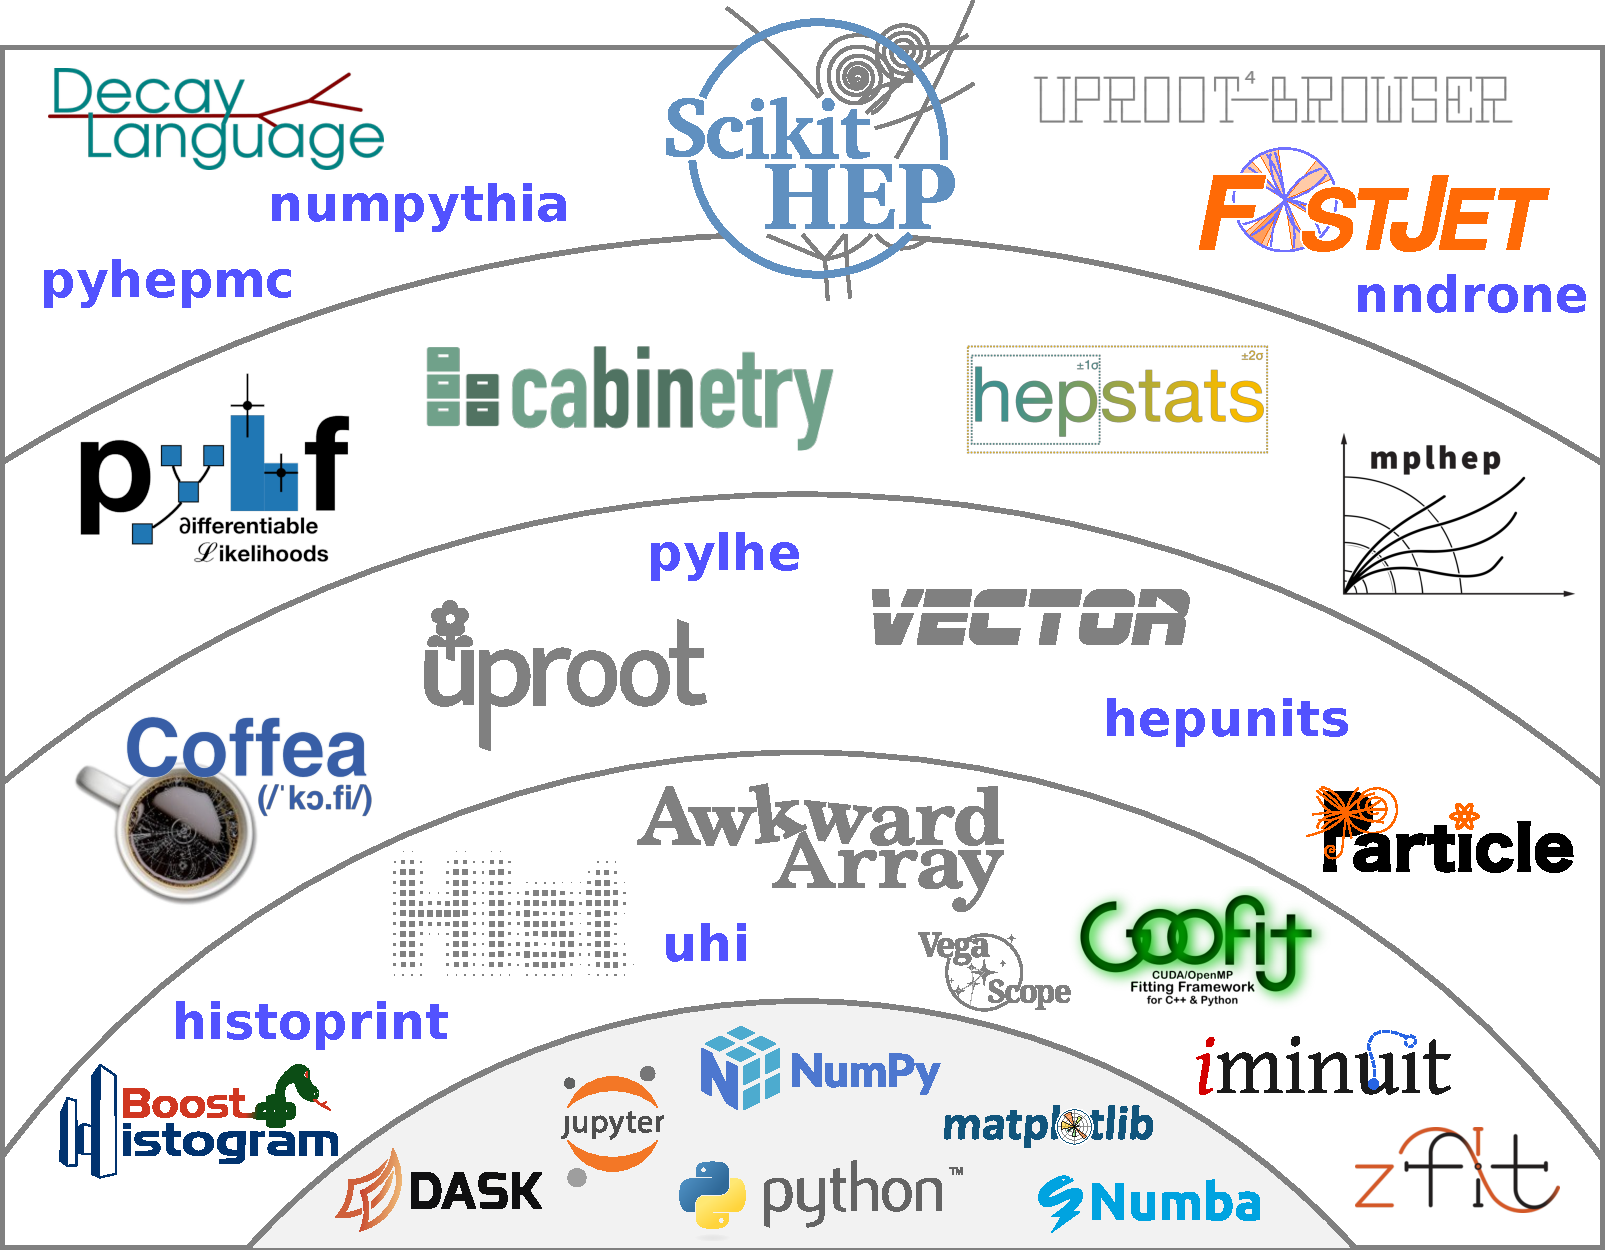
\includegraphics[width=\linewidth]{shells-hep.pdf}}
        \end{center}
    \end{figure}
  \end{columns}
\end{frame}
